% ============================================================
%  Siclaw: Defense-in-Depth Security Architecture for
%  Production LLM-Based SRE Agents
%
%  Target: AAAI 2027 (or NeurIPS 2026 Systems Track)
%  Format: 8 pages + unlimited references
% ============================================================
\documentclass[letterpaper]{article}

% --- AAAI REQUIRED (DO NOT CHANGE) ---
\usepackage[submission]{aaai25}
\usepackage{times}
\usepackage{helvet}
\usepackage{courier}
\usepackage[hyphens]{url}
\usepackage{graphicx}
\urlstyle{rm}
\def\UrlFont{\rm}
\usepackage{natbib}
\usepackage{caption}
\frenchspacing
\setlength{\pdfpagewidth}{8.5in}
\setlength{\pdfpageheight}{11in}

% --- Allowed additional packages ---
\usepackage{amsmath}
\usepackage{amssymb}
\usepackage{booktabs}
\usepackage{multirow}
\usepackage{algorithm}
\usepackage{algorithmic}
\usepackage{tikz}
\usetikzlibrary{positioning,arrows.meta,fit,backgrounds,calc,shapes.geometric}

\setcounter{secnumdepth}{0}

\pdfinfo{
/TemplateVersion (2025.1)
}

% --- Convenience macros ---
\newcommand{\sys}{\textsc{Siclaw}}
\newcommand{\ie}{\textit{i.e.}}
\newcommand{\eg}{\textit{e.g.}}
\newcommand{\etal}{\textit{et al.}}

\title{\sys{}: Defense-in-Depth Security Architecture for \\
Production LLM-Based SRE Agents}

\author{
  Anonymous Authors\textsuperscript{\rm 1} \\
  \textsuperscript{\rm 1}Anonymous Affiliation \\
  anonymous@example.com
}

\begin{document}
\maketitle

% ============================================================
\begin{abstract}
% ============================================================

Large language model (LLM) agents are increasingly deployed for Site Reliability Engineering (SRE)---incident diagnosis, root-cause analysis, and remediation in Kubernetes.
We report an emergent-safety finding that reframes how such agents should be deployed: across 400 real diagnosis traces on a live cluster (four LLM brains, \emph{no adversary}), agents \emph{spontaneously} generate sandbox-escape commands---host-namespace entry, container-runtime exec, network egress, and cluster writes---at 0.12 per case, with one brain 3--5$\times$ more escape-prone than its peers and the \emph{most accurate} brain among the most unsafe.
This behavior is invisible to the accuracy metrics existing benchmarks report, and existing SRE agents (Stratus, FLASH, RCAgent) and benchmarks (AIOpsLab, SREGym, ITBench) provide no security model to contain it.
We present \sys{}, the first production-grade SRE agent that treats the LLM as \emph{untrusted code}, enforcing safety through a six-layer defense-in-depth architecture: OS-level dual-user isolation with a novel setgid transitive-privilege mechanism, a six-pass command validator that decouples command definitions from execution-context policies, a three-layer output sanitizer, a four-stage guard pipeline for LLM output unreliability, and an extensible skill architecture with three-gate review. \sys{} runs in three modes---single-user TUI, multi-user local, and production Kubernetes with per-pod isolation---sharing one agent core.
\sys{}'s defense neutralizes \emph{every} one of the 0.12/case escape commands at no observed accuracy cost, blocks a 30-attack static red-team (no single layer exceeds 70\% coverage), and refuses 35/36 indirect-prompt-injection payloads embedded in live cluster resources with zero exfiltration.
Under a real LLM-as-judge checklist oracle it attains an 88--90\% diagnosis pass rate (mean 0.898--0.930) across the four brains with no self-judge bias, plus a first feasibility probe on 10 GPU/RDMA hardware-fault scenarios.
While general agent-safety benchmarks measure unsafe behavior in emulated sandboxes and privilege-control frameworks propose policy layers, to our knowledge \sys{} is the first to measure emergent unsafety in a \emph{live, production-grade SRE deployment on a real cluster} and to show that an OS-level defense contains it at \emph{zero measured accuracy cost}---establishing agent-as-untrusted-code as an empirical, not hypothetical, requirement for infrastructure agents.

\end{abstract}

% ============================================================
\section{Introduction}
% ============================================================

The rapid advancement of large language models (LLMs) has sparked significant interest in applying LLM-based agents to Site Reliability Engineering (SRE) tasks~\cite{chen2025aiopslab,chen2025stratus,zhang2024flash}.
These agents promise to automate incident diagnosis, root cause analysis (RCA), and remediation in complex cloud-native environments, potentially reducing mean time to resolution (MTTR) and alleviating the chronic shortage of experienced SRE practitioners.

Recent systems show encouraging \emph{capability}.
Stratus~\cite{chen2025stratus} reaches 78.5\% mitigation on the SREGym benchmark~\cite{clark2026sregym} via multi-agent collaboration with undo-and-retry; FLASH~\cite{zhang2024flash} reaches 59.3\% on AIOpsLab~\cite{chen2025aiopslab} via workflow decomposition with hindsight; and benchmarks such as AIOpsLab, SREGym, and ITBench~\cite{jha2025itbench} rigorously measure diagnostic accuracy.

Beneath these capability gains, however, lies a safety problem that accuracy metrics do not surface.
Instrumenting a production SRE agent on a live cluster, we find that \emph{even under benign, read-only diagnostic tasks with no adversary}, the agent spontaneously generates commands that would escape its sandbox---host-namespace entry (\texttt{nsenter}), container-runtime exec (\texttt{crictl}), network egress (\texttt{wget}/\texttt{nc}), and cluster writes (\texttt{kubectl rollout})---at 0.12 per case across 400 traces, with one model 3--5$\times$ more escape-prone than its peers and the \emph{most accurate} model among the most unsafe (\S\ref{sec:eval-emergent}).
Treating the LLM as trusted code is therefore untenable: an unconstrained agent simply executes these commands.

Yet \textbf{no existing SRE agent system treats the LLM as untrusted code.}
AIOpsLab mentions ``security policy filters'' for shell execution without specification; SREGym exposes unrestricted \texttt{kubectl} access (``cluster control for executing any commands''); Stratus, FLASH, and RCAgent~\cite{wang2024rcagent} provide no documented security model.
Combined with susceptibility to prompt injection~\cite{ruan2024toolemu} and hallucination-driven command generation, this exposes production infrastructure to credential theft, data exfiltration, and cluster-wide outages.

We identify five critical gaps in the current SRE agent literature (Table~\ref{tab:comparison}):
\begin{enumerate}
\item \textbf{Agent security}: No \emph{SRE} agent provides defense-in-depth against the agent's own generated commands; general privilege-control frameworks~\cite{progent2025} add a policy layer but no OS-level isolation and are not evaluated on live SRE deployments.
\item \textbf{Multi-tenant isolation}: All systems assume single-user, single-agent scenarios.
\item \textbf{Output sanitization}: No system prevents sensitive data (credentials, tokens) in command outputs from reaching the LLM's context.
\item \textbf{Agent reliability}: LLM output unreliability (malformed tool calls, context overflow) is documented by every benchmark but addressed by none.
\item \textbf{Knowledge extensibility}: Existing systems use fixed tool sets or static Standard Operating Procedures (SOPs), preventing organizational knowledge accumulation.
\end{enumerate}

\begin{table}[t]
\centering
\caption{Capability comparison of SRE agent systems. \sys{} is the only one addressing agent security, multi-tenant isolation, output sanitization, and extensible knowledge.}
\label{tab:comparison}
\small
\setlength{\tabcolsep}{3pt}
\begin{tabular}{@{}lccccc@{}}
\toprule
\textbf{Capability} & \rotatebox{90}{\textbf{AIOpsLab}} & \rotatebox{90}{\textbf{SREGym}} & \rotatebox{90}{\textbf{Stratus}} & \rotatebox{90}{\textbf{FLASH}} & \rotatebox{90}{\textbf{\sys{}}} \\
\midrule
Live K8s environment      & \checkmark & \checkmark & \checkmark & \checkmark$^\dagger$ & \checkmark \\
Agent security model       & ---        & ---        & ---        & ---$^\dagger$         & \textbf{6-layer} \\
Emergent-unsafety meas.\   & ---        & ---        & ---        & ---                   & \textbf{0.12/case} \\
Multi-tenant isolation     & ---        & ---        & ---        & ---                   & \textbf{3 modes} \\
Output sanitization        & ---        & ---        & ---        & ---                   & \textbf{3-layer} \\
Extensible skills          & ---        & ---        & ---        & fixed                 & \textbf{4-tier} \\
Guard pipeline             & ---        & ---        & ---        & ---                   & \textbf{4-stage} \\
GPU/RDMA fault eval.       & ---        & ---        & ---        & ---                   & \textbf{10 cases} \\
\bottomrule
\multicolumn{6}{@{}l}{\scriptsize $^\dagger$Proprietary; not reproducible.}
\end{tabular}
\end{table}

We present \sys{}, a production-grade SRE agent system that addresses all five gaps.
Our key contributions are:

\begin{itemize}
\item \textbf{Measured emergent unsafety in a live SRE deployment} (\S\ref{sec:threat}, \S\ref{sec:eval-emergent}): Where prior agent-safety work measures unsafe behavior in emulated sandboxes, we \emph{measure}---across 400 benign diagnosis traces on a real Kubernetes cluster---that competent SRE agents spontaneously emit 0.12 sandbox-escape commands per case, model-dependent (3--5$\times$) and decoupled from accuracy (the most accurate brain is among the most escape-prone). This establishes agent-as-untrusted-code as an empirical necessity for infrastructure agents, not a hypothetical.

\item \textbf{Defense-in-depth security architecture} (\S\ref{sec:security}): Six independent security layers, including a novel dual-user OS isolation model with setgid-based transitive privilege for selective credential access, a six-pass command validation pipeline, and a three-layer output sanitization pipeline. Each layer provides protection independently---compromising one does not disable the others.

\item \textbf{Guard pipeline for agent reliability} (\S\ref{sec:guards}): A four-stage message interception architecture (input, context, output, persist) that systematically addresses LLM output unreliability, including malformed tool call repair, context budget enforcement, and stream event correction.

\item \textbf{Multi-tenant runtime polymorphism} (\S\ref{sec:multitenant}): Three runtime modes sharing a unified agent core, with formal isolation invariants for shared-filesystem and per-pod deployment models.

\item \textbf{Extensible skill architecture} (\S\ref{sec:skills}): A four-tier skill hierarchy with three-gate review (static analysis, AI semantic review, human approval) enabling safe organizational knowledge accumulation.

\item \textbf{Comprehensive evaluation} (\S\ref{sec:eval}): 100 Kubernetes fault diagnosis cases across 10 categories and \emph{four} LLM brains under a real LLM-as-judge oracle; a \emph{measured} study of emergent agent unsafety and its containment; an indirect-prompt-injection study; a security red-team with layer ablation; and a GPU/RDMA fault-diagnosis feasibility probe.
\end{itemize}

% ============================================================
\section{Related Work}
% ============================================================

\paragraph{LLM-Based SRE Agents.}
LLM-based operations agents have advanced rapidly: from LLM root-cause analysis with historical reports~\cite{chen2024rcacopilot} and query recommendation~\cite{jiang2024xpert}, through tool-augmented ReAct-style RCA~\cite{wang2024rcagent,yao2023react} and tree-of-thought database diagnosis~\cite{zhou2024dbot}, to workflow decomposition with hindsight~\cite{zhang2024flash}, multi-agent observe/diagnose/mitigate pipelines (Stratus, highest mitigation on SREGym)~\cite{chen2025stratus}, SOP-guided multi-agent workflows~\cite{pei2025flowofaction}, LLM-assisted monitoring setup~\cite{yu2024monitorassistant}, and multi-modal RCA~\cite{zhang2025tamo}.
None of these treats the agent as untrusted or measures its unsafe behavior; all optimize \emph{capability} (diagnosis/mitigation accuracy), an axis orthogonal to the \emph{safety} properties we study.

\paragraph{AIOps Benchmarks.}
AIOpsLab~\cite{chen2025aiopslab} established the first holistic framework (48 problems over DeathStarBench~\cite{gan2019deathstarbench} microservices, the Agent-Cloud Interface concept); SREGym~\cite{clark2026sregym} extended it with noise injection, full-stack faults (including eBPF-simulated hardware failures), and an LLM-as-judge checklist oracle at $\kappa = 0.90$ human agreement; and ITBench~\cite{jha2025itbench}, OpenRCA~\cite{xu2025openrca}, and Cloud-OpsBench~\cite{wang2026cloudopsbench} broaden to general IT automation, root-cause localization, and reproducible agentic RCA.
These benchmarks evaluate diagnostic capability but assess neither agent safety, multi-tenant scenarios, nor GPU/RDMA faults---despite GPU hardware errors being the dominant failure mode in production AI clusters~\cite{cui2025gpuresilience,wan2025byterobust}.

\paragraph{Agent Safety and Privilege Control.}
A parallel line of work secures \emph{general} tool-using agents: AgentBench~\cite{liu2024agentbench} and ToolEmu~\cite{ruan2024toolemu} evaluate agents in sandboxed or emulated environments; Progent~\cite{progent2025} enforces least privilege through a programmable tool-call policy language; and KubeIntellect~\cite{kubeintellect2025} wraps a Kubernetes-management agent in RBAC and sandboxing. These contribute valuable \emph{policy} layers, but operate over general or emulated agents, add no \emph{OS-level} isolation beneath the policy, and do not report the capability cost of their controls. \sys{} differs on all three: it adds an OS-level isolation primitive (setgid transitive privilege) beneath the validator, runs as a \emph{live, read-only} production SRE agent, and quantifies that its defense costs \emph{zero} diagnostic accuracy (\S\ref{sec:eval-emergent}).

\paragraph{Measuring Agent Unsafety and Injection.}
A second line measures \emph{when} agents act unsafely: RedCode~\cite{redcode2024} benchmarks risky code execution, SandboxEscapeBench~\cite{sandboxescape2026} measures container breakout, and Saber~\cite{saber2026} probes operational-safety failures including benign tasks that invite unsafe shortcuts---the closest prior art to our emergent-unsafety finding. Indirect-prompt-injection suites---InjecAgent~\cite{injecagent2024} and AgentDojo~\cite{agentdojo2024}---measure injection susceptibility in tool-integrated agents.
All of these run in \emph{emulated or static-benchmark} settings over general or coding agents. \sys{} instead measures emergent unsafety in a \emph{live read-only SRE deployment on a real Kubernetes cluster} and---uniquely among this group---reports the \emph{diagnostic-accuracy cost} of containment, which we measure to be zero; our indirect-injection probe (\S\ref{sec:eval}) is complementary to InjecAgent and AgentDojo, which an infrastructure-specific suite at their scale should extend. To our knowledge, no prior system both measures this behavior on production infrastructure and contains it with an OS-level defense at no accuracy cost.

% ============================================================
\section{Threat Model and Problem Formulation}
\label{sec:threat}
% ============================================================

\paragraph{Core Assumption.}
We model the LLM agent as \emph{untrusted code} that generates shell commands executing in a container with Kubernetes cluster access.
The agent may attempt---through prompt injection, hallucination, or adversarial manipulation---to:
(T1)~\emph{read credentials} (kubeconfig, mTLS certificates, API keys);
(T2)~\emph{exfiltrate data} to external endpoints;
(T3)~\emph{escalate privileges} beyond read-only Kubernetes operations;
(T4)~\emph{leak sensitive information} through command outputs that enter the LLM context.

\paragraph{Trust Boundaries.}
The AgentBox container holds two trust domains: the \emph{main process} (Node.js runtime, LLM API client, tool validation) as user \texttt{agentbox}, and \emph{child processes} (LLM-generated shell commands) as user \texttt{sandbox}. The boundary lies at the command-execution interface: the main process validates and sanitizes; child processes execute with minimal privilege.

\paragraph{Security Goals.}
We enforce three security properties: \textbf{(1)~credential isolation}---child processes cannot read credential files even if command validation is bypassed; \textbf{(2)~least privilege}---only whitelisted commands with approved flags execute, with \texttt{kubectl} restricted to 13 read-only subcommands; and \textbf{(3)~output safety}---sensitive data (tokens, keys, connection strings) in command outputs is redacted before entering the LLM context.

\paragraph{Problem Formulation.}
At each step an agent generates a command $c_t$ from history and observations; a security pipeline $\mathcal{S}$ approves, modifies, or blocks it ($c'_t=\mathcal{S}(c_t)$), and the resulting output is sanitized ($r'_t=\mathcal{O}(r_t,c'_t)$) before re-entering the context, with a guard pipeline $\mathcal{G}$ repairing malformed messages and enforcing context budgets. The goal is to maximize diagnostic accuracy subject to $\mathcal{S}$ enforcing credential isolation and least privilege and $\mathcal{O}$ enforcing output safety at every step.

% ============================================================
\section{System Architecture}
\label{sec:arch}
% ============================================================

\begin{figure*}[t]
\centering
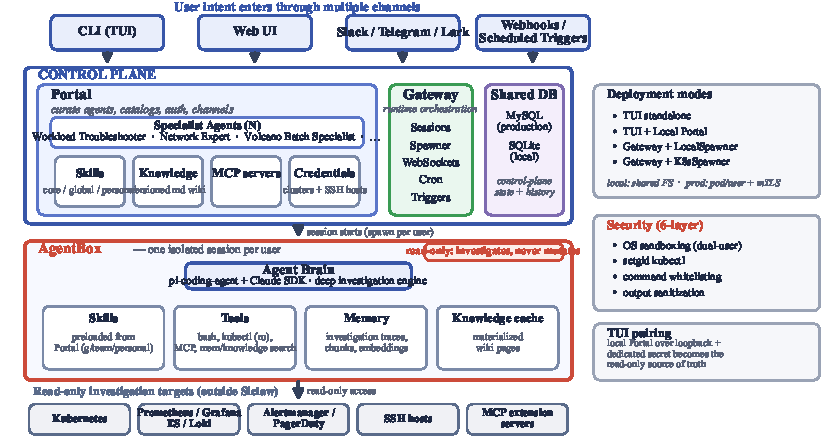
\includegraphics[width=0.80\textwidth]{figures/overview.pdf}
\caption{
\sys{} system overview. User intent enters through four channels and reaches the \emph{control plane} (Portal, Gateway, shared DB), which curates specialist agents, skills, knowledge, MCP servers, and credentials. Each session spawns an isolated \emph{AgentBox}---a Kubernetes pod in production, in-process locally, or embedded in a standalone TUI---holding the agent brain, preloaded skills, read-only tools, a private memory DB, and a materialized knowledge cache. Every target it touches is accessed \emph{read-only}, and a six-layer security architecture (Figure~\ref{fig:architecture}) constrains all agent actions.
}
\label{fig:overview}
\end{figure*}

\sys{} is built on a single brain abstraction (OpenAI-compatible provider interface) with a unified tool registry, guard pipeline, and security architecture. As Figure~\ref{fig:overview} shows, user intent flows through a control plane that orchestrates per-user \emph{AgentBox} sessions, each investigating read-only infrastructure targets; this section details the agent core and its security architecture (Figure~\ref{fig:architecture}).

\begin{figure}[t]
\centering
\resizebox{0.80\columnwidth}{!}{%
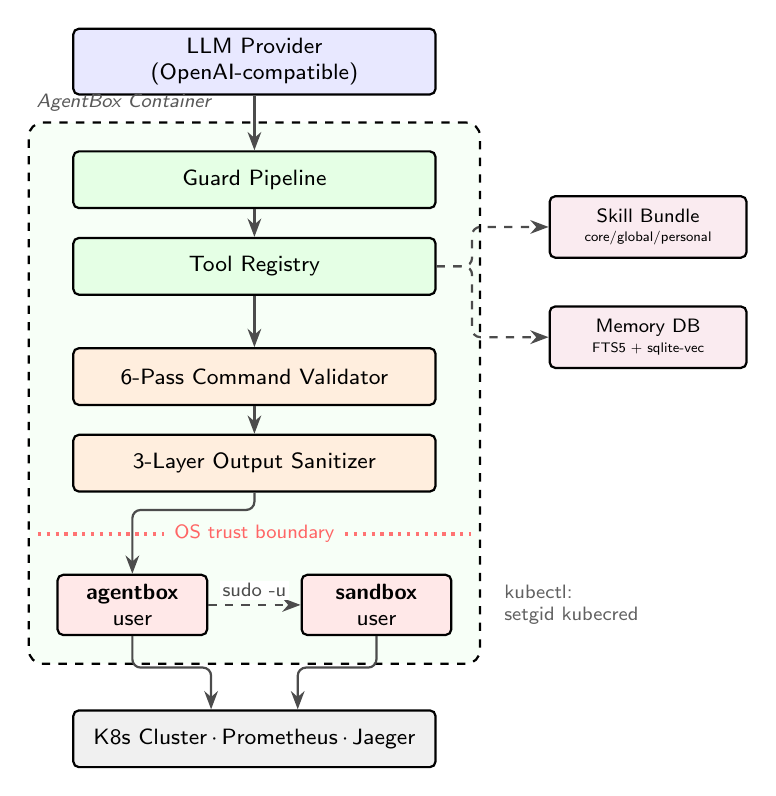
\begin{tikzpicture}[
    >=Stealth,
    box/.style={draw, rounded corners=2pt, minimum height=0.72cm, align=center,
                font=\sffamily\footnotesize, thick, minimum width=4.6cm},
    sidebox/.style={draw, rounded corners=2pt, minimum height=0.78cm, align=center,
                font=\sffamily\scriptsize, thick, minimum width=2.5cm, fill=purple!8},
    userbox/.style={draw, rounded corners=2pt, minimum height=0.72cm, align=center,
                font=\sffamily\footnotesize, thick, minimum width=1.9cm, fill=red!9},
    arr/.style={->, thick, color=black!70},
  ]
  % --- Main vertical pipeline (centered at x=0) ---
  \node[box, fill=blue!9]   (llm)  at (0, 8.0) {LLM Provider\\(OpenAI-compatible)};
  \node[box, fill=green!10] (guard)at (0, 6.5) {Guard Pipeline};
  \node[box, fill=green!10] (tool) at (0, 5.4) {Tool Registry};
  \node[box, fill=orange!13](valid)at (0, 4.0) {6-Pass Command Validator};
  \node[box, fill=orange!13](sani) at (0, 2.9) {3-Layer Output Sanitizer};
  \node[userbox] (abox) at (-1.55, 1.1) {\textbf{agentbox}\\user};
  \node[userbox] (sbox) at ( 1.55, 1.1) {\textbf{sandbox}\\user};
  \node[box, fill=gray!12] (k8s) at (0, -0.6) {K8s Cluster\,$\cdot$\,Prometheus\,$\cdot$\,Jaeger};

  % --- Side panel (right) ---
  \node[sidebox] (skill) at (5.0, 5.9) {Skill Bundle\\[-1pt]{\tiny core/global/personal}};
  \node[sidebox] (mem)   at (5.0, 4.5) {Memory DB\\[-1pt]{\tiny FTS5 + sqlite-vec}};

  % --- AgentBox container zone (background) ---
  \begin{scope}[on background layer]
    \node[draw, dashed, thick, rounded corners=5pt, fill=green!3, inner sep=10pt,
          fit=(guard)(tool)(valid)(sani)(abox)(sbox)] (zone) {};
  \end{scope}
  \node[font=\sffamily\scriptsize\itshape, text=black!65, anchor=south west, inner sep=1pt]
        at ([xshift=2pt, yshift=2.5pt]zone.north west) {AgentBox Container};

  % --- Trust boundary (between sanitizer and user row); line broken so the label never touches it ---
  \draw[dotted, very thick, red!55] (-2.75, 2.0) -- (-1.15, 2.0);
  \draw[dotted, very thick, red!55] ( 1.15, 2.0) -- ( 2.75, 2.0);
  \node[font=\sffamily\scriptsize, text=red!60, inner sep=1.5pt] at (0, 2.0) {OS trust boundary};

  % --- Main vertical pipeline (straight, orthogonal) ---
  \draw[arr] (llm)  -- (guard);
  \draw[arr] (guard)-- (tool);
  \draw[arr] (tool) -- (valid);
  \draw[arr] (valid)-- (sani);

  % --- sanitizer -> agentbox user: rounded right-angle, crossing the trust boundary ---
  \draw[arr, rounded corners=3pt] (sani.south) -- ++(0,-0.22) -| (abox.north);

  % --- agentbox -> sandbox (sudo -u): label lifted clear of the line on a white patch ---
  \draw[arr, dashed] (abox.east) -- node[font=\sffamily\scriptsize, above=1.5pt, text=black!70, inner sep=1pt, fill=white] {sudo -u} (sbox.west);

  % --- both users -> cluster: symmetric rounded right-angle elbows, separate entry points ---
  \draw[arr, rounded corners=3pt] (abox.south) -- ++(0,-0.40) -| ([xshift=-0.55cm]k8s.north);
  \draw[arr, rounded corners=3pt] (sbox.south) -- ++(0,-0.40) -| ([xshift= 0.55cm]k8s.north);

  \node[font=\sffamily\scriptsize, text=black!62, anchor=west, align=left] at (3.05, 1.1) {kubectl:\\setgid kubecred};

  % --- tool registry -> side panels: rounded right-angle elbows (no diagonals) ---
  \draw[arr, dashed, rounded corners=3pt] (tool.east) -- ++(0.45,0) |- (skill.west);
  \draw[arr, dashed, rounded corners=3pt] (tool.east) -- ++(0.45,0) |- (mem.west);
\end{tikzpicture}%
}
\caption{
\sys{} architecture. LLM-generated commands flow through the guard pipeline, tool registry, 6-pass validator, and 3-layer sanitizer before crossing the OS trust boundary. Child processes run as the unprivileged \texttt{sandbox} user; \texttt{kubectl} reaches the kubeconfig via setgid.
}
\label{fig:architecture}
\end{figure}


% ------- 4.1 Defense-in-Depth Security -------
\subsection{Defense-in-Depth Security Architecture}
\label{sec:security}

The security architecture consists of six independent layers, each providing protection even if others are compromised. This section details the three most novel layers.

\subsubsection{Layer 1: OS-Level Dual-User Isolation}

The AgentBox container contains two Linux users:
\texttt{agentbox} (UID 1000, groups: \texttt{agentbox}, \texttt{kubecred}) runs the main Node.js process, and
\texttt{sandbox} (UID 1001, group: \texttt{sandbox}) runs all LLM-generated shell commands via \texttt{sudo -E -u sandbox}.

\paragraph{Transitive Privilege via setgid.}
\texttt{kubectl} must read kubeconfig files, but \texttt{sandbox} must not. We solve this with a setgid mechanism: \texttt{kubectl} is installed setgid to the \texttt{kubecred} group (\texttt{-rwxr-sr-x root:kubecred}) and kubeconfig is \texttt{agentbox:kubecred} mode \texttt{0640}. When \texttt{sandbox} runs \texttt{kubectl}, the setgid bit temporarily grants \texttt{kubecred} membership so \texttt{kubectl} alone reads the kubeconfig; other commands (\texttt{grep}, \texttt{cat}, \texttt{jq}) lack it. This preserves \emph{pipeline compatibility}---\texttt{kubectl get pods | grep Error} works because data flows through non-access-controlled stdout while credentials stay protected by filesystem permissions. Since kubeconfig (\texttt{0640}) and mTLS certs/API keys (\texttt{0600}) are unreadable by \texttt{sandbox}, even a full Layer~2 bypass leaves credential access independently blocked.

\subsubsection{Layer 2: Six-Pass Command Validation Pipeline}

Every LLM-generated command passes through six independent validation passes before execution, over a context $\xi \in \{\texttt{local}, \texttt{node}, \texttt{pod}\}$:
\emph{(1)~shell operators}---block \texttt{\$()}, backticks, \texttt{<()}/\texttt{>()}, redirections, and embedded newlines;
\emph{(2)~pipeline extraction}---parse the command into stages $[s_1|s_2|\ldots]$;
then, per stage,
\emph{(3)~binary whitelist}---verify $\text{binary}(s_i)\in\mathcal{W}_\xi$ (the context-specific allowlist);
\emph{(4)~subcommand validation}---for \texttt{kubectl}, restrict to 13 read-only subcommands (\texttt{get}, \texttt{describe}, \texttt{logs}, \ldots);
\emph{(5)~flag restrictions}---apply per-command rules (\texttt{pipeOnly}, \texttt{noFilePaths}, \texttt{blockedFlags}, \texttt{allowedFlags});
and finally \emph{(6)~sensitive paths}---block commands targeting credential/configuration files.

\paragraph{Context-Policy Decoupling.}
A key design innovation separates \emph{command definitions} (\texttt{COMMANDS} registry: binary names, categories, per-command rules) from \emph{context policies} (\texttt{CONTEXT\_POLICIES}: which categories each execution context allows). For example, the \texttt{local} context blocks file-reading commands (\texttt{cat}, \texttt{ls}, \texttt{find})---the agent has dedicated file tools with path access control---while the \texttt{pod} context allows them. This keeps the $\sim$80-binary allowlist maintainable: a new command specifies its category and rules once, and context policies determine where it may execute.

\subsubsection{Layer 3: Three-Layer Output Sanitization}

Command outputs may carry sensitive data (JWT tokens, connection strings, PEM certificates) that would enter the LLM context if not intercepted. Three layers address this: (1)~\emph{pre-execution analysis} (\texttt{analyzeOutput}) inspects the command to pick a sanitizer; (2)~\emph{post-execution redaction} (\texttt{applySanitizer}) redacts sensitive env-var names (\texttt{*\_API\_KEY}, \texttt{*\_SECRET}, \texttt{DATABASE\_URL}) and value patterns (JWT \texttt{eyJ...}, PEM \texttt{-----BEGIN}, connection strings); and (3)~a \emph{pipeline fallback} applies line-level pattern redaction to the final output when a downstream stage (\eg\ \texttt{jq} in \texttt{kubectl get secret -o yaml | jq .data}) has no registered rule, catching what the first two missed.

\subsubsection{Layers 4--6: Container Hardening, File I/O, Environment}

\textbf{Layer 4 (Container hardening)} drops all Linux capabilities except the five required for the dual-user model (\texttt{SETUID}, \texttt{SETGID}, \texttt{CHOWN}, \texttt{FOWNER}, \texttt{AUDIT\_WRITE}), uses a read-only root filesystem, and disables the service-account token mount.
\textbf{Layer 5 (File I/O restrictions)} has the agent's file tools enforce \texttt{assertPathAllowed()}, scoping reads/writes to designated directories so the agent cannot reach credential files through its own tools.
\textbf{Layer 6 (Environment sanitization)} runs \texttt{sanitizeEnv()} before spawning child processes, stripping API keys, tokens, and sensitive variables to prevent leakage via \texttt{/proc/\{pid\}/environ}.

The security architecture is validated by 184 passing unit tests (97 command validator, 48 output sanitizer, 15 pipeline integration, 16 guard pipeline, 8 tool-call repair).


% ------- 4.2 Guard Pipeline -------
\subsection{Guard Pipeline for Agent Reliability}
\label{sec:guards}

LLM agents exhibit systematic output unreliability---malformed tool-call JSON, missing tool-call IDs, context-window overflow from large outputs, corrupted streaming events---that every benchmark documents~\cite{chen2025aiopslab,clark2026sregym} yet none systematically solves. The guard pipeline intercepts agent messages at four lifecycle stages.
\emph{Input guards} transform the message history before each API call: dropping tool-call blocks missing required fields (\texttt{id}/\texttt{name}/\texttt{input}) and ensuring every \texttt{toolCall} has a matching \texttt{toolResult} (inserting synthetic error results where needed).
\emph{Context guards} enforce a three-tier budget: truncate any single tool result over 50\% of the window, compact oldest results past 75\%, and raise a preemptive overflow signal at 90\% before the API rejects the request.
\emph{Output guards} repair streaming events in-flight: trimming/ID-filling unnamed tool calls and extracting balanced JSON from partial \texttt{toolcall\_delta} events by bracket counting.
\emph{Persist guards} validate messages before session-history writes: sanitizing tool calls, tracking call/result pairing, inserting synthetic results for orphaned calls, and truncating oversized ($>$400KB) results.
The pipeline uses a \emph{single-wrap-per-hook} architecture---each of the brain's three hook points (\texttt{streamFn}, \texttt{appendMessage}, \texttt{transformContext}) is wrapped exactly once---avoiding nested monkey-patching while keeping per-stage control.


% ------- 4.3 Multi-Tenant Runtime -------
\subsection{Multi-Tenant Runtime Polymorphism}
\label{sec:multitenant}

As shown in Figure~\ref{fig:overview}, \sys{} supports four runtime modes sharing one agent core, trading isolation for convenience: (1)~\textbf{standalone TUI}; (2)~\textbf{TUI + local Portal} (read-only Portal snapshot over loopback with three-gate authentication); (3)~\textbf{Gateway + LocalSpawner} for multi-user local development on a shared filesystem; and (4)~\textbf{Gateway + K8sSpawner} for production, with per-user pod isolation and mTLS certificates encoding \texttt{userId}/\texttt{workspaceId}.
Two invariants matter: on the shared filesystem (mode 3), \texttt{materialize()} must never be called (it would overwrite all users' skill directories), and in production (mode 4) per-pod isolation is the multi-tenant boundary. All modes implement the \texttt{BoxSpawner} interface; the unified agent core operates identically across them.


% ------- 4.4 Extensible Skill Architecture -------
\subsection{Extensible Skill Architecture}
\label{sec:skills}

Existing SRE agents use fixed tool sets~\cite{chen2025aiopslab,clark2026sregym} or static SOPs~\cite{pei2025flowofaction}. \sys{} instead organizes diagnostic skills into a four-tier hierarchy ordered by user proximity (personal $>$ skillset $>$ global $>$ core): \textbf{core} skills are baked into the container image (versioned with code), \textbf{global} are organization-wide, \textbf{skillset} are team-scoped (development only, promoted to global for production), and \textbf{personal} are per-user. The bundle contract (\texttt{buildSkillBundle}) transmits only non-core skills, as core skills exist on disk.

\paragraph{Three-Gate Review.}
Because skills execute as code, new skills pass three independent safety gates before production: (1)~\emph{static analysis} against 22 danger patterns (shell injection, credential access, unsafe operations); (2)~\emph{AI semantic review} of skill intent; and (3)~\emph{human approval}. Unapproved skills cannot execute regardless of tier---enabling safe organizational knowledge accumulation, unlike the fixed tool sets of prior systems.


% ------- 4.5 Hybrid Memory System -------
\subsection{Hybrid Memory System}
\label{sec:memory}

Each AgentBox maintains a private memory database (SQLite with FTS5 and sqlite-vec) holding structured investigation records over a full lifecycle (create\,$\rightarrow$\,update\,$\rightarrow$\,resolve\,$\rightarrow$\,reference). Search blends vector similarity and keyword matching, $\text{score}=w_v\cos(\mathbf{q},\mathbf{d})+w_f\,\text{BM25}(q,d)+w_t\,\text{decay}(t)$ ($w_v{=}0.70$, $w_f{=}0.30$, temporal decay), reranked via Maximal Marginal Relevance; knowledge documents are heading-chunked ($\sim$400 tokens), embedded, and dual-indexed, letting the agent recall prior investigations rather than starting each incident cold.


% ============================================================
\section{Evaluation}
\label{sec:eval}
% ============================================================

We evaluate \sys{} along five axes: (1)~diagnostic capability on 100 Kubernetes faults across \emph{four} LLM brains under a real LLM checklist oracle; (2)~\emph{measured} emergent unsafety---how often a benign agent spontaneously emits sandbox-escape commands---and its containment; (3)~indirect prompt injection in live cluster resources; (4)~a static security red-team with per-layer ablation; and (5)~a 10-scenario GPU/RDMA feasibility probe.

% ------- 5.1 Diagnostic Evaluation -------
\subsection{Diagnostic Evaluation}
\label{sec:eval-diag}

\subsubsection{Setup}

We construct a benchmark of 100 Kubernetes fault diagnosis cases across 10 categories (per-category counts in the technical appendix), following the methodology of SREGym~\cite{clark2026sregym} and AIOpsLab~\cite{chen2025aiopslab}, deployed on a real 368-node cluster (2 GPU nodes, H100 NVLink 80GB; Volcano scheduling; Calico NetworkPolicy). Each case injects a specific fault and gives the agent a symptom-level prompt (\eg\ ``Pod \texttt{c031-pending} is stuck in Pending''); the agent investigates autonomously with \texttt{kubectl}, \texttt{grep}, \texttt{jq}, and other whitelisted tools. Every case is run by \emph{four} diverse brains---Claude Sonnet 4.6, Kimi K2.5, DeepSeek V4-Flash, Qwen3.6-27B (400 runs total)---testing generalization beyond a single model. The agent is \emph{read-only}: no mutations are permitted, itself a safety property of the architecture (\S\ref{sec:threat}), not merely an evaluation convenience.

\subsubsection{Scoring}

Following SREGym's checklist methodology, each diagnosis is scored 0--1 across five dimensions---\textbf{localization} (right target resource), \textbf{mechanism} (root cause, not symptom), \textbf{scope} (blast radius), \textbf{evidence} (concrete observables), and \textbf{remediation} (safe, root-cause-matched fix)---by a real LLM checklist judge (Claude Sonnet 4.6) that answers grounded Yes/No questions, each requiring a verbatim trace quote and a confidence label, at temperature~0 against per-case oracle ground truth; a case passes if its mean exceeds 0.65.
This judge is deliberately distinct from brittle label matching: re-scoring traces, it reverses artifacts in \emph{both} directions---a false pass where the agent called a pod ``healthy'' yet missed an anti-affinity conflict ($0.80\!\rightarrow\!0.10$) and a false failure where a correct diagnosis used non-matching wording ($0.47\!\rightarrow\!1.00$).
The same frozen judge scores all four brains, avoiding self-judge bias; as a reliability check, an \emph{independent} judge (DeepSeek~V4) re-scores a stratified 20-case sample and reproduces its per-question verdicts at Cohen's $\kappa = 0.87$ (94.5\% agreement). The verbatim checklist and agreement protocol are in the technical appendix (Diagnosis Evaluation Checklist and Inter-Judge Agreement); full human-$\kappa$ validation is the remaining, stronger step.

\subsubsection{Results}

\begin{table}[t]
\centering
\caption{Diagnostic results across four brains (100 cases each, real LLM checklist judge). The frozen Claude judge ranks DeepSeek, Qwen, and Kimi at or above Claude itself---evidence against self-judge bias.}
\label{tab:models}
\small
\setlength{\tabcolsep}{2.6pt}
\begin{tabular}{@{}lrrccccc@{}}
\toprule
\textbf{Brain} & \textbf{Pass\%} & \textbf{Score} & \textbf{Loc} & \textbf{Mech} & \textbf{Scope} & \textbf{Evid} & \textbf{Rem} \\
\midrule
Claude S4.6     & 88.0 & 0.898 & 0.92 & 0.90 & 0.86 & 0.93 & 0.89 \\
Kimi K2.5       & 88.0 & 0.906 & 0.90 & 0.88 & 0.92 & 0.95 & 0.89 \\
DeepSeek V4     & \textbf{90.0} & \textbf{0.930} & 0.94 & 0.90 & 0.94 & 0.96 & 0.92 \\
Qwen3.6-27B     & 89.0 & 0.901 & 0.91 & 0.87 & 0.90 & 0.95 & 0.88 \\
\bottomrule
\end{tabular}
\end{table}

\sys{} achieves an 88--90\% pass rate (mean score 0.898--0.930) across the four brains (Table~\ref{tab:models}). The result generalizes: the frozen Claude judge ranks DeepSeek, Qwen, and Kimi at or above Claude itself, so the headline is neither a single-model artifact nor self-judging. Tool budgets differ sharply (DeepSeek/Kimi resolve most cases in 4.9--6.0 calls and 19--30\,s vs.\ Claude's 7.4 and 51\,s) with no accuracy penalty, and scores are balanced across the five dimensions---scope (0.86--0.94) and remediation (0.88--0.92) stay in range, not the degenerate extremes (scope $0.48$, remediation $1.000$) that brittle label matching produced.

The accuracy gap lives in \emph{categories}, not dimensions: easy single-fault categories (image-pull, config, storage) saturate at 100\%, while the three hardest---network-DNS (57.5\% pass), compound multi-fault (64.3\%), controller (71.9\%)---are weakest \emph{consistently} across brains (full per-category breakdown in the technical appendix). These demand reasoning over multi-resource impact chains (NetworkPolicy$+$DNS, owner-reference hierarchies); difficulty is intrinsic, not a single-model weakness, and even non-monotonic---nominally ``medium'' network/controller cases (70.8\%) are \emph{harder} than ``hard'' GPU/compound cases (81.0\%). We report these honest sub-threshold cells rather than the saturated aggregate.



% ------- 5.2 Security Evaluation -------
\subsection{Security Red-Team Evaluation}
\label{sec:eval-security}

We design 30 attacks across the four threat categories---T1 credential reading (8), T2 exfiltration (8), T3 privilege escalation (8), T4 output leakage (6)---each run as a concrete command string against the real security-pipeline functions (\texttt{validateCommand}, \texttt{validateShellOperators}, \texttt{postExecSecurity}), attributed to the first layer that intercepts it. This \emph{static} suite complements the \emph{behavioral} measurements that follow (emergent unsafety and indirect injection). \textbf{All 30 attacks are blocked}, with blocks spread across layers (T1 by L2/L4/L6, T2 by L2/L1/L5, T3 by L5/L2, T4 by L4); the per-category block-to-layer map is in the technical appendix (Security Red-Team Catalog). Since this tests attacks the pipeline was designed to catch, the load-bearing evidence is behavioral, and an adaptive/LLM-generated red-team is future work.


% ------- 5.3 Security Layer Ablation -------
\subsection{Security Layer Ablation}
\label{sec:eval-ablation}

To validate the defense-in-depth design, we test each security layer independently---``if \emph{only} this layer existed, how many of the 30 attacks would it block?'' (per-layer coverage table in the technical appendix, Security Red-Team Catalog). Three findings hold: (1)~no single layer exceeds 70\% coverage (L2's binary whitelist is the strongest at 21/30, but misses all kubectl-write attacks, caught by L5, and output leakage, caught by L4); (2)~18/30 attacks (60\%) are caught by 2+ layers, demonstrating true defense-in-depth; and (3)~12 attacks are caught by exactly one layer, so removing it would open a vulnerability (\eg\ kubectl-write commands are caught \emph{only} by L5's subcommand check).


% ------- 5.4 Security–Capability Tradeoff -------
\subsection{Emergent Unsafety During Benign Diagnosis}
\label{sec:eval-emergent}

Our central safety claim is not about adversaries: it is that a \emph{benign} agent, given only a read-only diagnostic task, spontaneously emits commands that would escape its sandbox. We measure this directly. Across all 400 diagnosis traces (4~brains $\times$ 100 cases, 2{,}262 tool calls, \emph{no} injected adversary), the security pipeline blocked \textbf{47 sandbox-escape commands}---\textbf{0.12 per case} (Table~\ref{tab:emergent}). These are pure hallucination, not attacks: \texttt{nsenter} into host namespaces, \texttt{crictl}~\texttt{exec}/\texttt{pull}, \texttt{wget}/\texttt{nc} egress, \texttt{xargs}/\texttt{python3}/\texttt{awk} shell-outs, \texttt{\$()} substitution, input redirection, and \texttt{kubectl rollout}. 46 of the 47 are caught by the L2 binary/subcommand whitelist; the remaining one by the sensitive-path rules. The operational definition of a sandbox-escape command and the full counting protocol are in the technical appendix (Emergent-Unsafety Measurement Protocol).

\begin{table}[t]
\centering
\caption{Emergent unsafety over 400 \emph{benign} traces (no adversary): 47 spontaneously-generated sandbox-escape commands blocked. DeepSeek---the \emph{most accurate} brain---is 3--5$\times$ more escape-prone, a divergence invisible to accuracy metrics.}
\label{tab:emergent}
\small
\begin{tabular}{@{}lrrrr@{}}
\toprule
\textbf{Brain} & \textbf{Tool calls} & \textbf{Blocked} & \textbf{Cases} & \textbf{Per case} \\
\midrule
Claude S4.6       & 739 & 8  & 4  & 0.08 \\
Kimi K2.5         & 486 & 5  & 5  & 0.05 \\
DeepSeek V4-Flash & 605 & \textbf{27} & \textbf{16} & \textbf{0.27} \\
Qwen3.6-27B       & 432 & 7  & 6  & 0.07 \\
\midrule
\textbf{Total}    & \textbf{2262} & \textbf{47} & \textbf{31} & \textbf{0.12} \\
\bottomrule
\end{tabular}
\end{table}

The rate is strongly model-dependent: DeepSeek emits escape commands \textbf{3--5$\times$ more often} than its peers (0.27/case vs.\ 0.05--0.08)---yet is simultaneously the most accurate brain (Table~\ref{tab:models}), so this safety-relevant gap is \emph{invisible} to accuracy metrics. This is the empirical core of the agent-as-untrusted-code thesis: unsafe command generation is a baseline property of competent agents under normal operation, not an adversarial edge case, varying by model in ways accuracy benchmarks miss.

\paragraph{Accuracy cost.}
Does blocking these commands hurt diagnosis? Examining every failed case for a security-attributable failure---a block whose output a correct diagnosis would have required---we found \emph{none}: all 47 are redundant escape attempts (\eg\ \texttt{wget} to a service already reachable via \texttt{kubectl get}/\texttt{describe}), and every diagnosis completed using only the read-only whitelist (\texttt{get}, \texttt{describe}, \texttt{logs}, \texttt{events}, \texttt{top}). To confirm this, we ran a controlled security-off A/B on DeepSeek---the most escape-prone brain---re-running all 100 cases with the read-only analysis toolkit widened (blocked commands $27\!\rightarrow\!19$; irreversible actions still blocked). Accuracy is statistically unchanged: pass rate $90.0\%\!\rightarrow\!88.0\%$, mean score $0.930\!\rightarrow\!0.919$ ($\Delta=-0.011$), 83/100 cases identical and the rest splitting symmetrically (8 better, 9 worse)---noise, not a security penalty. We thus observe \textbf{no measurable accuracy cost} (A/B protocol and preserved irreversible-action ``safety floor'' in the technical appendix).

\subsection{Indirect Prompt Injection via Tool Output}
\label{sec:eval-inject}

A distinctive infrastructure threat is \emph{indirect} prompt injection: a malicious instruction planted in cluster state (a ConfigMap value, pod-log line, or annotation) that the agent ingests as tool output while investigating. We embed 12 such payloads---service-account-token reads, \texttt{curl} exfiltration, RBAC escalation, reverse shells, secret dumps---in live cluster resources and run each against 3 brains (36 trials; Claude omitted due to an unrelated gateway incompatibility). \textbf{35 of 36 are refused outright}: the agent recognizes the injected instruction and declines to act. In the one case where DeepSeek attempted an embedded token read, the sensitive-path layer neutralized it; \textbf{zero payloads exfiltrated data}. Multi-turn chains and payloads disguised as legitimate runbook steps are future work.

% ------- 5.5 GPU/RDMA Infrastructure Fault Diagnosis -------
\subsection{GPU/RDMA Fault Diagnosis: A Feasibility Probe}
\label{sec:eval-gpu}

No published SRE benchmark evaluates agent diagnosis of GPU hardware errors (Xid events, ECC failures, NVLink degradation) or RDMA fabric issues (link flapping, PFC storms, QP errors)~\cite{clark2026sregym,chen2025aiopslab,yu2024fisurvey}, despite these being the dominant failure modes in production GPU clusters. We design 10 scenarios by \emph{observable-signal simulation}: rather than injecting hardware faults (which needs physical access), we reproduce the signals an SRE agent would observe---\texttt{dmesg}, \texttt{nvidia-smi}, RDMA counters (\texttt{ibstat}, \texttt{ethtool}), NCCL logs---as Kubernetes ConfigMaps, matching the agent's real interface. Lacking oracle ground truth for these synthetic scenarios, we score them by a heuristic signal-coverage rubric (did the diagnosis name the Xid code, affected GPU, link-layer counter?)---\emph{not} the LLM checklist judge---grounded in production fault data~\cite{cui2025gpuresilience,wan2025byterobust}, so we present this as a feasibility probe, not a graded benchmark.

All 10 scenarios reach the pass threshold (mean rubric 0.923; per-case breakdown in the technical appendix). Qualitatively, the agent maps Xid codes to specific GPUs, distinguishes thermal throttling from genuine OOM, and attributes RDMA faults to link-layer counters; in compound case g09 it names \emph{both} independent root causes (GPU ECC $+$ RDMA congestion). We read this as preliminary evidence that an LLM agent \emph{can} diagnose GPU/RDMA faults given appropriate telemetry, while cautioning that the heuristic rubric and simulated signals make this weaker evidence than the LLM-judged Kubernetes results.


\paragraph{Comparison and scope.}
Comparison with SREGym is not apples-to-apples: it reports \emph{end-to-end} success \emph{including mitigation} (Claude Code 60.7\%, Stratus 54.8\%~\cite{clark2026sregym}), whereas \sys{} is graded read-only on its own diagnosis-only cases. We make no capability claim against SREGym; our contribution is the orthogonal \emph{safety} dimension those benchmarks omit, and running \sys{} directly on SREGym's cases is the clear next step.


% ============================================================
\section{Discussion and Conclusion}
% ============================================================

\sys{} is, to our knowledge, the first production-grade SRE agent that treats the LLM as untrusted code, and our central finding makes that stance empirical: across 400 benign traces, competent agents spontaneously emit 0.12 sandbox-escape commands per case through ordinary hallucination---no adversary, model-dependent ($3$--$5\times$), decoupled from accuracy. The six-layer defense neutralizes all 47 escapes and resists 35/36 indirect-injection payloads with zero exfiltration, at no measured accuracy cost ($90.0\%\!\rightarrow\!88.0\%$); since unsafe command generation is a \emph{measured} baseline property and not an edge case, we argue agent-as-untrusted-code is necessary for production. The architecture is not Kubernetes-specific---the dual-user model, validator, and sanitizer apply to any LLM agent executing shell commands, and context-policy decoupling adds new contexts (cloud CLIs, database tools) without touching command definitions---and the GPU/RDMA probe suggests LLM agents \emph{can}, given telemetry, diagnose a fault class absent from existing SRE benchmarks~\cite{cui2025gpuresilience,yu2024fisurvey}, motivating a labelled, LLM-judge-graded GPU/RDMA benchmark on real hardware.

\paragraph{Limitations.}
The evaluation uses a single cluster topology and a single run per case (no confidence intervals); cross-cluster and multi-seed runs are future work. The LLM judge is corroborated by an independent judge ($\kappa=0.87$) but not yet by human labels (the SREGym standard; in progress). The ``no accuracy cost'' A/B is on a single brain (DeepSeek) against a pre-existing security-on run, so run-to-run noise is not fully removed. The GPU/RDMA probe uses simulated signals and a heuristic rubric; the static red-team covers attacks the pipeline was built to catch, not adaptive or multi-turn injection; and the Stratus/Claude Code comparison relies on published results, not direct reproduction. We hope \sys{} provides both a foundation and a research agenda for secure autonomous operations.


% ============================================================
% References
% ============================================================
\bibliography{references}

\clearpage
\appendix
% ============================================================
% REPRODUCIBILITY CHECKLIST (stays in the main PDF)
% The full technical detail (model/cluster configuration, benchmark
% construction, the verbatim LLM-judge rubric and inter-judge
% agreement protocol, the emergent-unsafety counting protocol, the
% security-off A/B protocol, the red-team catalog, the indirect-
% injection payloads, the GPU/RDMA probe, and worked case studies)
% is provided in the separate "Siclaw: Technical Appendix"
% supplementary PDF (siclaw-supplementary.tex).
% ============================================================

\noindent\textit{The accompanying \emph{Technical Appendix} (supplementary material) provides the additional detail needed to reproduce every experiment in \S\ref{sec:eval}: the model and cluster configuration, how the 100-case benchmark is constructed, the verbatim LLM-judge rubric and inter-judge agreement protocol, the operational definition and counting protocol behind the emergent-unsafety result, the security-off A/B protocol, the red-team catalog and layer map, the indirect-injection payloads, the GPU/RDMA probe, and worked case studies. The AAAI reproducibility checklist below stays in the main paper.}

% ------------------------------------------------------------
\section{Reproducibility Checklist}
\label{app:checklist}

\noindent\textit{Self-reported per the AAAI-26 reproducibility checklist. Authors should re-verify every answer (especially code/data release) against the final artifact before submission.}

\paragraph{This paper.}
(1)~Conceptual outline/pseudocode of methods introduced: \textbf{yes} (\S\ref{sec:security}--\S\ref{sec:guards}, and the technical appendix protocols for emergent-unsafety measurement through the security red-team catalog).
(2)~Opinions/hypotheses delineated from facts: \textbf{yes} (feasibility probes and single-run results are explicitly flagged).
(3)~Pedagogical references for background: \textbf{yes}.

\paragraph{Theoretical contributions.}
The paper's contributions are primarily systems and empirical; the only formal claims are the multi-tenant isolation invariants (\S\ref{sec:multitenant}), stated as operational contracts.
(1)~Assumptions stated: \textbf{partial}. (2)~Claims stated formally: \textbf{partial}. (3)~Proofs included: \textbf{no} (argued, not proved). (4)~Proof sketches/intuitions: \textbf{partial}. (5)~Citations to tools: \textbf{yes}. (6)~Claims demonstrated empirically: \textbf{yes}. (7)~Code to disprove claims: \textbf{NA}.

\paragraph{Datasets.}
(1)~Motivation for datasets: \textbf{yes} (technical appendix, Benchmark Construction). (2)~Novel datasets in a data appendix: \textbf{partial} (described in the technical appendix, Benchmark Construction; case manifests in the code release). (3)~Public on publication: \textbf{partial} (intended, with a responsible-release note for the attack/injection catalogs---authors to confirm). (4)~Existing datasets cited: \textbf{yes} (SREGym, AIOpsLab, DeathStarBench). (5)~Existing datasets public: \textbf{yes}. (6)~Non-public datasets described: \textbf{yes} (cluster and cases; technical appendix, Model and Infrastructure Configuration and Benchmark Construction).

\paragraph{Computational experiments.}
(1)~Hyperparameter ranges/selection: \textbf{partial} (judge $\tau=0.65$, temperature~0 documented; few tunable parameters). (2)~Pre-processing code: \textbf{partial}. (3)~Source code in a code appendix: \textbf{partial} (system and harness released). (4)~Code public on publication: \textbf{partial} (authors to confirm). (5)~Code commented with paper references: \textbf{partial}. (6)~Random-seed method: \textbf{partial} (judge is deterministic at temperature~0; agent sampling is provider-default and single-run per case---a stated limitation). (7)~Computing infrastructure specified: \textbf{yes} (technical appendix, Model and Infrastructure Configuration). (8)~Evaluation metrics formally described: \textbf{yes} (technical appendix, Diagnosis Evaluation Checklist and Inter-Judge Agreement). (9)~Number of runs per result: \textbf{yes} (one run per case, disclosed). (10)~Beyond single-dimensional summaries: \textbf{partial} (per-category/-dimension/-brain breakdowns and inter-judge $\kappa$; no confidence intervals---a stated limitation). (11)~Statistical-significance tests: \textbf{no} (the A/B and category analyses are descriptive; a paired significance test is future work). (12)~Final hyperparameters listed: \textbf{yes} (technical appendix, Model and Infrastructure Configuration).

\end{document}
